\begin{prob}[3.2]
  Solve the optimal activity level problem described in exercise 4.7 in Convex
  Optimizaiton, for the instance with problem data
  \[
  A = \begin{bmatrix}
    1 & 2 & 0 & 1\\
    0 & 0 & 3 & 1\\
    0 & 3 & 1 & 1\\
    2 & 1 & 2 & 5\\
    1 & 0 & 3 & 2\\
  \end{bmatrix},
  c^{\max} = \begin{bmatrix}
    100\\
    100\\
    100\\
    100\\
    100
  \end{bmatrix},
  p = \begin{bmatrix}
    3\\
    2\\
    7\\
    6\\
  \end{bmatrix},
  p^{disc} = \begin{bmatrix}
    2\\
    1\\
    4\\
    2\\
  \end{bmatrix},
  q = \begin{bmatrix}
    4\\
    10\\
    5\\
    10\\
  \end{bmatrix}
  \]
\end{prob}

You can do this by forming the LP you found in your solution of exercise 4.17, or more directly,
using CVX. Give the optimal activity levels, the revenue generated by each one, and the total
revenue generated by the optimal solution. Also, give the average price per unit for each activity
level, i.e., the ratio of the revenue associated with an activity, to the activity level. (These
numbers should be between the basic and descounted prices for each activity.) Give a very brief
story explaining, or at least commenting on, the solution you find. \textbf{You also need to
  submit your CVX matlab code.}
\begin{proof}[\sol]
  \verbatiminput{source/h3q2.m}
  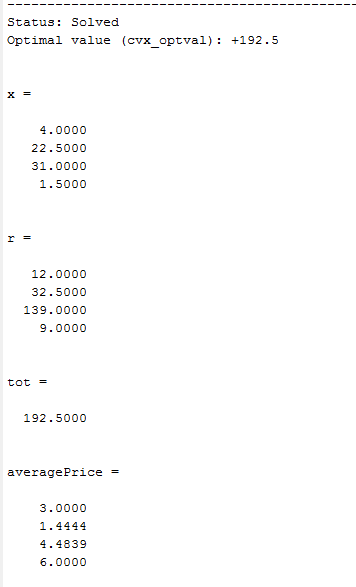
\includegraphics{source/h3qq2}

  When performing the above calculations, we should take note that our 3rd value for $x$ is the highest. Now, from the original matrices, we will note that this activity level also has a high discounted price, also the value for the average price is higher than the discount price, thus it contributes to the total more.  Next we will note that the value for the last activity has a discounted price which is substantially lower then the basic price. Here we use of a lot of resources and therefore its activity level is low.
\end{proof}
